\documentclass[a4]{article}
\usepackage{geometry}
\geometry{verbose,tmargin=2.5cm,bmargin=2.5cm,lmargin=3cm,rmargin=3cm}
\usepackage{amsmath,amssymb,amsthm}
\usepackage{graphicx}
\graphicspath{{graphics/}}
\usepackage[utf8]{inputenc}
\usepackage{fancyvrb}
\usepackage{hyperref}
\usepackage{lscape}
\usepackage{adjustbox}
\usepackage{verbatim}
\usepackage{subcaption}
\usepackage{placeins}

\title{MultiFEBE \\ Tutorial 6: static analysis of a floating pile with boundary elements and finite elements}
\author{\'A.G. Vega-Artiles}
\date{September 2022}

\begin{document}

\maketitle

\tableofcontents 

\section{Problem description}

In this sixth tutorial, the horizontal pressure distribution along different floating piles due to a static load is obtained using the BEM-FEM coupling. The results can be directly compared against the literature \cite{poulos}, which serves as a validation case for this coupled model.

A floating pile is a foundation with a slender cylindrical shape which is buried into the soil. The structure is mainly one-dimensional, thus it is modelled as a finite element region consisting on beam finite elements. The soil is a half-space (unbounded domain) and it is modelled as a boundary element region. For this boundary element region, the half-space Green's function (Mindlin solution) is used, so no discretization is needed for the free-surface. The soil-pile interaction is introduced by including in the boundary element region a body line load whose discretization must be conforming to the beam finite elements. Figure \ref{fig:layout} shows the devised mesh for the problem.

\begin{figure}[tbh!]
	\centering
	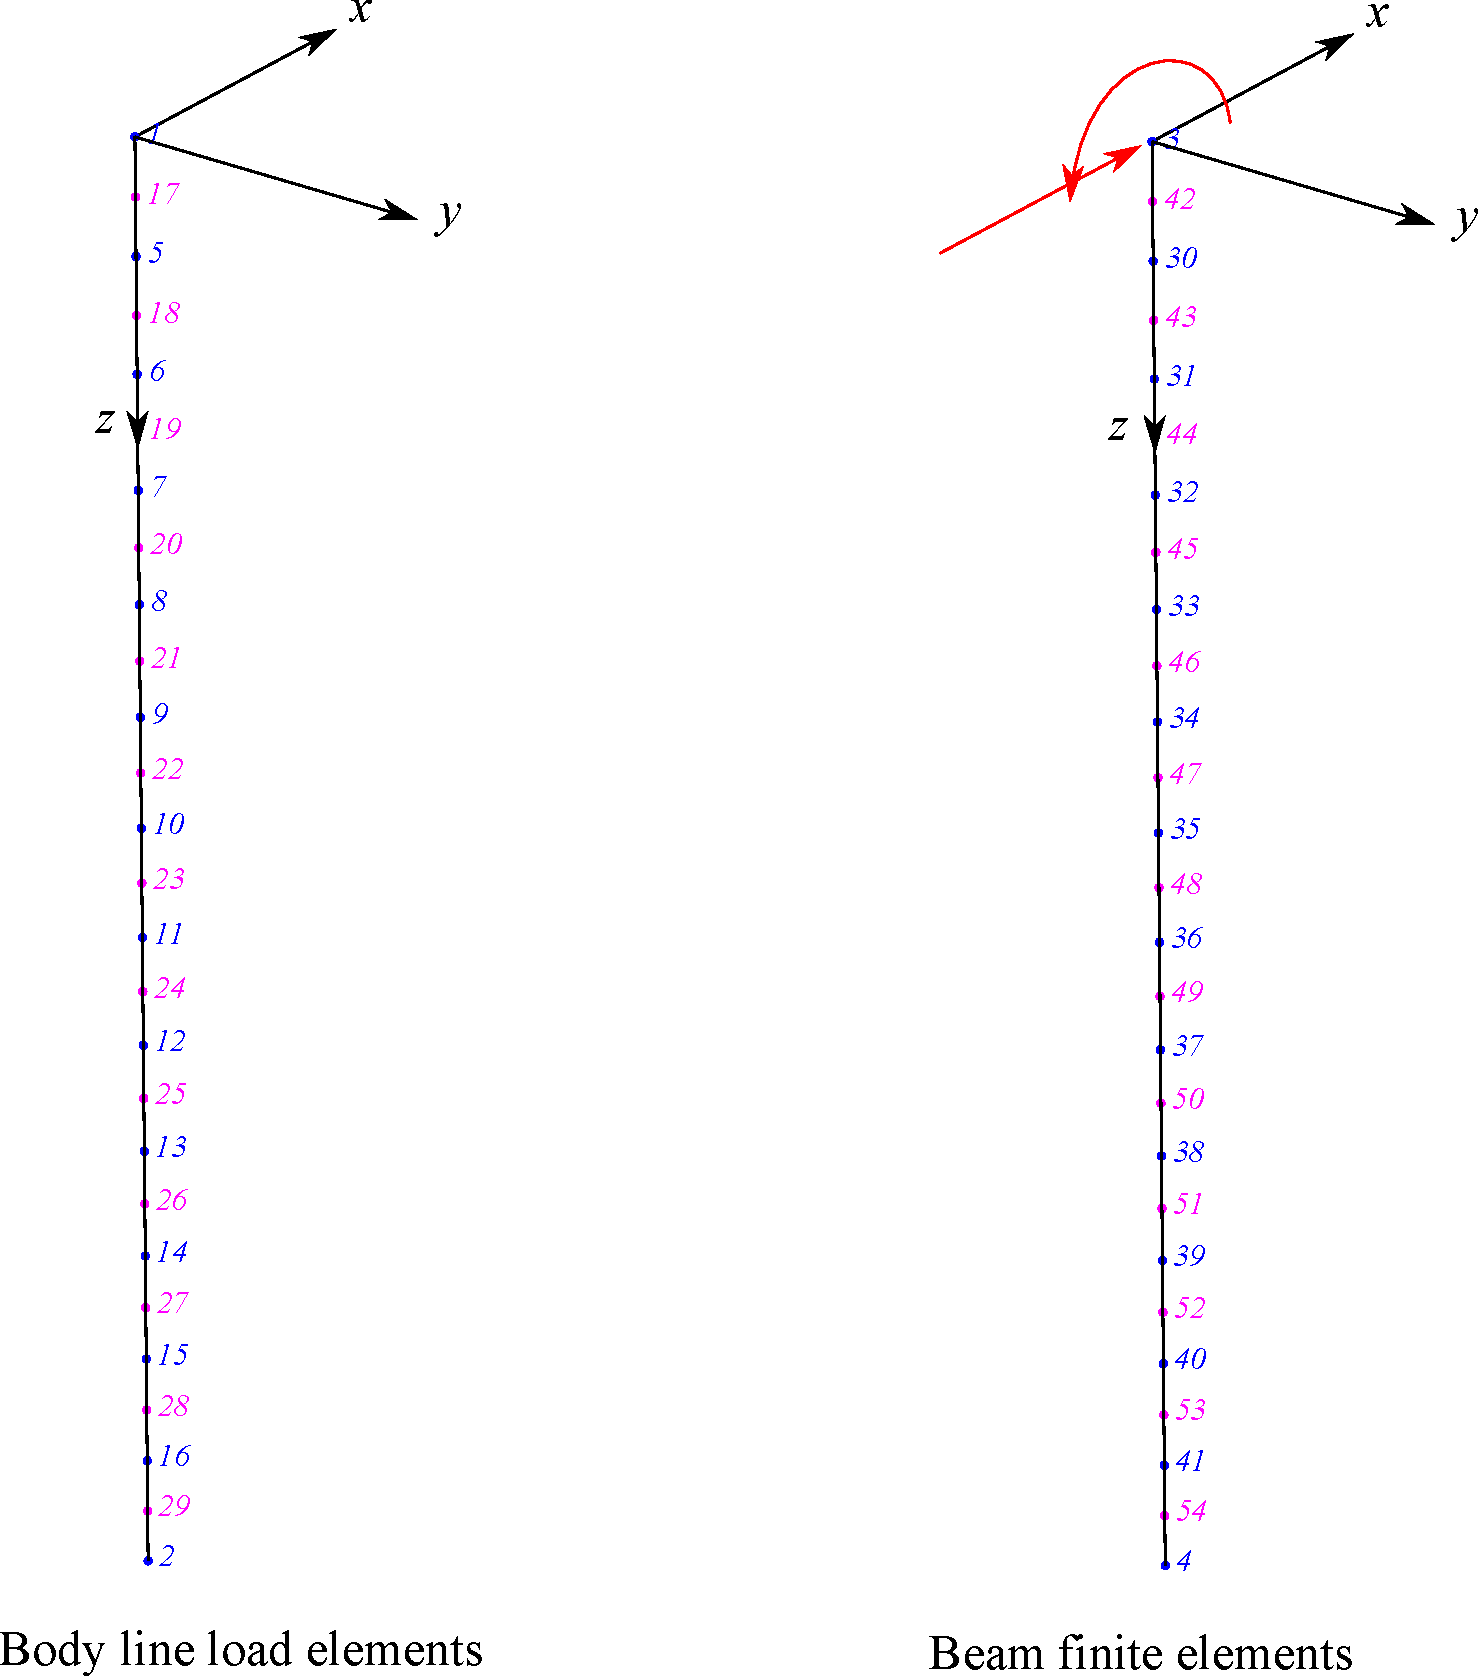
\includegraphics[scale=0.4]{floating.pdf}
	\caption{Mesh for the floating pile example. Boundary element mesh consists only on body line load elements, which geometrically coincides to beam finite element mesh.}
	\label{fig:layout}
\end{figure}

\section{Pre-processing} 
Pre-processing in MultiFEBE consists of defining the geometry and mesh of the problem. There are three ways to do such definition: directly from the input file (mode = 0), from another file in the native format (mode = 1) or from another file in the Gmsh MSH file format version 2.2 (mode = 2). However, it is preferable to use a *.msh file for relatively large geometries, therefore, this is the syntax explained in the following subsections.
   
\subsection{Mesh generation with Gmsh}
Gmsh \cite{gmsh, gmshweb} is a finite element mesh generator with its own language. The software allows to create the geometry in a “bottom-up” manner, going from the most basic elements (points) to the highest order elements (volumes) or in a “Constructive Solid Geometry” manner (boolean operations) or with a combination of methodologies. Gmsh also allows to define  the so-called “physical groups” which are unmodifiable entities that gather elementary entities as sole entities, where every entity must have a unique tag. On the other hand, the file containing all this geometric definition is the *.geo file whereas the mesh definition is in the *.msh file. 

\subsubsection{GEO file}
The Gmsh language allows to define parameters to use later in the script and comments as every other programming language. 

In this example two parameters are defined: the pile length (Lpile) and the mesh element size (ms\_pile). Every point in the geometry can be specified by its coordinates (x y z) and the mesh element size to use there with the function ``Point". Every straight line of the model is created with the function ``Line" and its initial and final points. Then, with the function ``Physical Line" every line is converted into a single entity or physical entity with its own name. The function ``Transfinite Line" explicitly defines the location of the nodes on the line by following the expression specified and the function ``Ceil" rounds up values to the nearest integer. Furthermore, it is worth noting that “if an expression defines a new entity, it is enclosed between parentheses but if an expression refers to a previously defined entity, it is enclosed between braces.” \cite{gmshweb}

Finally, the mesh generation, the element order and the *.msh file saving can also be specified with the expressions ``Mesh + mesh dimension", ``SetOrder + element order" and ``Save + name.msh”,
respectively.

The resulting *.geo file applied to the problem is the following:

\begin{Verbatim}
// Geometry & mesh parameters
Lpile = 25;
ms_pile = 2;

Point (1) = {0, 0, 0, ms_pile};
Point (2) = {0, 0, Lpile, ms_pile};
Line  (1) = {1, 2};
Transfinite Line {1} = Ceil(Lpile/ms_pile + 1.);
Physical Line ("line-load") = {1};

Point (3) = {0, 0, 0, ms_pile};
Point (4) = {0, 0, Lpile, ms_pile};
Line  (2) = {3, 4};
Transfinite Line {2} = Ceil(Lpile/ms_pile + 1.);
Physical Line ("pile") = {2};

// Mesh generation
Mesh 1;
SetOrder 2;
Save "mesh.msh";
\end{Verbatim}

\subsubsection{MSH file}

The *.msh file begins with a mandatory section about information of the file (MeshFormat) and following by the other sections. Here, three sections are used: the physical group names (PhysicalName), the nodes (Nodes) and the elements (Elements).

In the section ``PhysicalName", all the physical entities of the model are defined. The first line indicates the number of physical entities. Then, one line per physical entity indicating the physical dimension, the tag and the name.  

In the section ``Nodes", all the nodes of the model are defined. The first line indicates the number of nodes. Then, one line per node indicating the node identifier and its coordinates (x y z).

In the section ``Elements", all the elements of the model are defined. The first line indicates the number of elements. Then, one line per element indicating:

\begin{itemize}
	\item Element identifier.
	\item Type of element.
	\item Number of auxiliary tags.
	\item List of tags, where the two first auxiliary tags are mandatory, and the first one corresponds to the identifier of the physical entity to which the element belongs and the second one is the identifier of the elementary model entity to which the element belongs. The rest of the tags are optional.
	\item A list of identifiers corresponding to the nodes of the element.
\end{itemize}

For example, in this case, an element with the identifiers 1 8 2 1 1 1 5 7 corresponds to:

\begin{itemize}
	\item 1: element 1.
	\item 8: type 8 (3-node second order line).
	\item 2: it has 2 auxiliary tags.
	\item 1: it belongs to the physical entity 1.
	\item 1: it belongs to the line 1.
	\item 1, 5, 7: it connects the nodes 1, 5 and 7.
\end{itemize} 

Finally, the *.msh file can be obtain in \textit{File $\to$ Export}.

The resulting *.msh file applied to the problem is the following:

\begin{Verbatim}
$MeshFormat
2.2 0 8
$EndMeshFormat

$PhysicalNames
2
1 1 "line-load"
1 2 "pile"
$EndPhysicalNames

$Nodes
54
1 0 0 0
2 0 0 25
3 0 0 0
4 0 0 25
5 0 0 1.923076923069284
6 0 0 3.846153846138358
7 0 0 5.769230769205297
8 0 0 7.692307692272241
9 0 0 9.615384615345244
10 0 0 11.53846153841902
11 0 0 13.4615384614928
12 0 0 15.38461538456658
13 0 0 17.30769230765023
14 0 0 19.23076923073767
15 0 0 21.15384615382511
16 0 0 23.07692307691256
17 0 0 0.9615384615346747
18 0 0 2.884615384604353
19 0 0 4.807692307671953
20 0 0 6.730769230738639
21 0 0 8.653846153808447
22 0 0 10.57692307688226
23 0 0 12.4999999999539
24 0 0 14.42307692302983
25 0 0 16.34615384610878
26 0 0 18.26923076919312
27 0 0 20.19230769228153
28 0 0 22.11538461536667
29 0 0 24.03846153845748
30 0 0 1.923076923069284
31 0 0 3.846153846138358
32 0 0 5.769230769205297
33 0 0 7.692307692272241
34 0 0 9.615384615345244
35 0 0 11.53846153841902
36 0 0 13.4615384614928
37 0 0 15.38461538456658
38 0 0 17.30769230765023
39 0 0 19.23076923073767
40 0 0 21.15384615382511
41 0 0 23.07692307691256
42 0 0 0.9615384615346747
43 0 0 2.884615384604353
44 0 0 4.807692307671953
45 0 0 6.730769230738639
46 0 0 8.653846153808447
47 0 0 10.57692307688226
48 0 0 12.4999999999539
49 0 0 14.42307692302983
50 0 0 16.34615384610878
51 0 0 18.26923076919312
52 0 0 20.19230769228153
53 0 0 22.11538461536667
54 0 0 24.03846153845748
$EndNodes

$Elements
26
1 8 2 1 1 1 5 17
2 8 2 1 1 5 6 18
3 8 2 1 1 6 7 19
4 8 2 1 1 7 8 20
5 8 2 1 1 8 9 21
6 8 2 1 1 9 10 22
7 8 2 1 1 10 11 23
8 8 2 1 1 11 12 24
9 8 2 1 1 12 13 25
10 8 2 1 1 13 14 26
11 8 2 1 1 14 15 27
12 8 2 1 1 15 16 28
13 8 2 1 1 16 2 29
14 8 2 2 2 3 30 42
15 8 2 2 2 30 31 43
16 8 2 2 2 31 32 44
17 8 2 2 2 32 33 45
18 8 2 2 2 33 34 46
19 8 2 2 2 34 35 47
20 8 2 2 2 35 36 48
21 8 2 2 2 36 37 49
22 8 2 2 2 37 38 50
23 8 2 2 2 38 39 51
24 8 2 2 2 39 40 52
25 8 2 2 2 40 41 53
26 8 2 2 2 41 4 54
$EndElements
\end{Verbatim}

\subsection{Input data file}
Solving in MultiFEBE consists of running the software by specifying several options in the following sections\footnote{See reference manual.}: [problem], [settings], [materials], [regions], [conditions over nodes], etc.

The first part to configurate is the problem definition in the section [problem]. This example is a 3D static mechanical problem.

\begin{Verbatim}	
[problem]
n = 3D
type = mechanics
analysis = static
\end{Verbatim}

In the section [export], several export settings are defined. In this example, the nodal solutions and the stress resultant solutions will be exported by writing the option T with the corresponding expression, ``export\_nso" and ``export\_tot", respectively.

\begin{Verbatim}
[export]
export_nso = T
export_tot = T
\end{Verbatim}

Next step is to configurate the mesh. In this case, a mesh from Gmsh will be used so that it is necessary to write the option number 2 and the document name obtained from it in the section [settings]. However, if the mesh were going to be read from the input file, it would require to write the sections [nodes], [elements] and [parts] instead.

\begin{Verbatim}	
[settings]
mesh_file_mode = 2 "mesh.msh"
\end{Verbatim}

As the problem has two materials, the section [materials] will need three lines: a first line for the number of materials in the model and a line per material with its properties such as tag, type, E and $\nu$.

\begin{Verbatim}
[materials]
2
1 elastic_solid E 200.d6 nu 0.49d0
2 elastic_solid E 182.4214d9 nu 0.3d0
\end{Verbatim}

In the section [be body loads], all body loads in BE regions are defined. The format consists of a first line with the number of BE body loads to be defined, next as many lines as BE body loads. Each line contains first the BE body load identifier and last the mesh part which contains the elements associated with it.

\begin{Verbatim}
[be body loads]
1
1 1
\end{Verbatim}

The section [fe subregions] indicates the number of fe subregions in the first line (1) and a line per subregions indicating the subregion identifier (1) and the part identifier (2). The last two zeros at the end are mandatory and they are going to be used in the future for additional features.

\begin{Verbatim}
[fe subregions]
1
1 2 0 0
\end{Verbatim}

In the section [cross sections], it is necessary to specify the number of cross sections in the first line and a line per cross section by indicating the type of fe (strbeam\_t = straight beam, Timoshenko model), number of fe subregions related to the cross section (1), fe subregion identifier (1), type of cross section (circle), radius (1.) and reference vector for the section orientation (1. 0. 0.).

\begin{Verbatim}
[cross sections]
1
strbeam_t 1 1 circle 1. 1. 0. 0.
\end{Verbatim}

The format of the section [regions] consists of a first line indicating the number of regions (2). Furthermore, for each region there must be a block of data consisting of several lines. 

The first region is a BE half-space, so the region identifier and the region class (discretization method) are \emph{1 be}. Then, as a half-space the following data specify:

\begin{itemize}
	\item -3: The normal vector to the surface is in -z direction.
	\item 0.: Coordinate of the free surface.
	\item 1: Boundary condition of the free surface. Free traction in this case. 
\end{itemize}

The second line indicates the number of boundaries and a list of boundaries (0), the third line defines the material (material 1) and the fourth line defines the number and list of BE body loads (1 1).

The second region is a FE region, so the first line shows the region identifier and the region class (discretization method) (2 fe). Then, the second line indicates the number of subregions (1) and their identifiers (1) and the third line the material (material 2). 

\begin{Verbatim}	
[regions]
2

1 be half-space -3 0. 1
0
material 1
1 1

2 fe
1 1
material 2
\end{Verbatim}

In the section [conditions over nodes], all boundary conditions over nodes will be specified. As a 3D model, there are 6 lines for every boundary condition. Every line has two digits, where the first one indicates the type of condition (0 for displacement and 1 for force) and the second one the value. In case of displacement, firstly the displacements $u_x, u_y, u_z$ are configured and then the rotations $\theta_x, \theta_y, \theta_z$. In case of force, firstly the forces $F_x, F_y, F_z$ and then the moments $M_x, M_y, M_z$. 

\begin{Verbatim}	
[conditions over nodes]
node 3: 1 1.
        1 0.
        1 0.
        1 0.
        1 0.
        1 0.
\end{Verbatim}

The whole data file applied to the problem is the following:

\begin{Verbatim}
[problem]
n = 3D
type = mechanics
analysis = static

[export]
export_nso = T
export_tot = T

[settings]
mesh_file_mode = 2 "mesh.msh"

[materials]
2
1 elastic_solid E 200.d6 nu 0.49d0
2 elastic_solid E 182.4214d9 nu 0.3d0

[be body loads]
1
1 1

[fe subregions]
1
1 2 0 0

[cross sections]
1
strbeam_t 1 1 circle 1. 1. 0. 0.

[regions]
2

1 be half-space -3 0. 1
0
material 1
1 1

2 fe
1 1
material 2

[conditions over nodes]
node 3: 1 1.
        1 0.
        1 0.
        1 0.
        1 0.
        1 0.
\end{Verbatim}

\section{Results and discussion}

Figure \ref{fig:results} shows the dimensionless pressure along a floating pile for several cases. The results from \cite{poulos} are shown together with the obtained results from the present model. The cases differ in pile slenderness $L=D$ ($ L $ is the pile length and $ D $ is the pile diameter), pile head constraints (free-head or fixed-head where rotation is constrained), loading type (horizontal force $ F_x $ or moment $ M_y $), and pile flexibility factor $ K_R = E_pI_p=(E_sL^4) $. It is observed a very good agreement except around the pile tip and head, where small discrepancies appear presumably due to the simplification introduced by a one-dimensional modelling of the pile-soil interaction.

\begin{figure}[tbh!]
	\centering
	\begin{subfigure}[b]{0.48\textwidth}
		\centering
		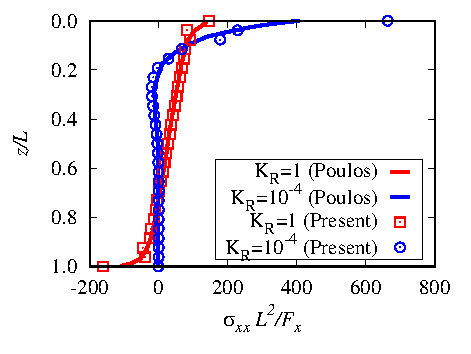
\includegraphics[width=\textwidth]{floating_a.eps}
		\caption{Free-head and horizontal load $F_x$ applied. Pile with $L/D=25$, and soil $\nu_s=0.5$.}
		\label{fig:floating_results_a}
	\end{subfigure}
	\begin{subfigure}[b]{0.48\textwidth}
		\centering
		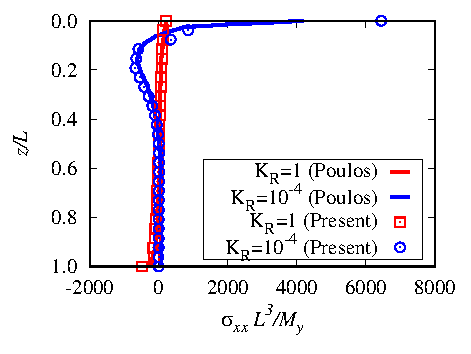
\includegraphics[width=\textwidth]{floating_b.eps}
		\caption{Free-head and moment load $M_y$ applied. Pile with $L/D=25$, and soil $\nu_s=0.5$.}
		\label{fig:floating_results_b}
	\end{subfigure}
	\begin{subfigure}[b]{0.48\textwidth}
		\centering
		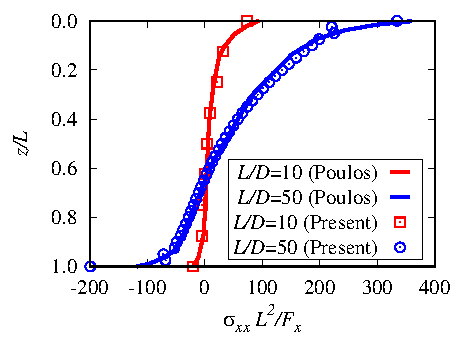
\includegraphics[width=\textwidth]{floating_c.eps}
		\caption{Free-head and horizontal load $F_x$ applied. Pile flexibility $K_R=0.01$, and soil $\nu_s=0.5$.}
		\label{fig:floating_results_c}
	\end{subfigure}
	\begin{subfigure}[b]{0.48\textwidth}
		\centering
		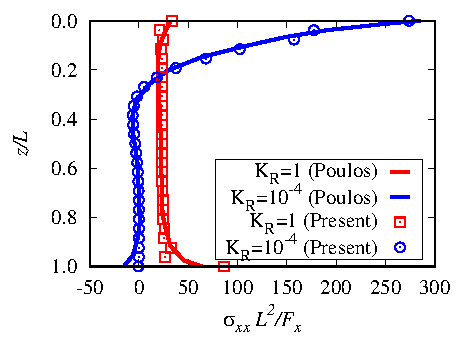
\includegraphics[width=\textwidth]{floating_d.eps}
		\caption{Fixed-head and horizontal load $F_x$ applied. Pile with $L/D=25$, and soil $\nu_s=0.5$.}
		\label{fig:floating_results_d}
	\end{subfigure}    
	\caption{Pressure distribution along floating piles for several  cases. Reference results are taken from \cite{poulos}.}
	\label{fig:results}
\end{figure}

\FloatBarrier

\begin{thebibliography}{99}
	
	\bibitem{poulos} H. G. Poulos and E. H. Davis. ``Elastic solutions for soil and rock mechanics." \textit{Centre for Geotechnical Research}, (1991).

	\bibitem{gmsh} C. Geuzaine and J.-F. Remacle, ``Gmsh: a three-dimensional finite element mesh generator with built-in pre- and post-processing facilities." \textit{International Journal for Numerical Methods in Engineering}, Volume 79, Issue 11, pages 1309--1331, (2009).
	
	\bibitem{gmshweb} C. Geuzaine and J.-F. Remacle, ``Gmsh." \url{http://gmsh.info/}

\end{thebibliography}

\end{document}
